\begin{frame}
  \frametitle{Robust MLMs}

  \begin{itemize}
  \item \proglang{R} has a large collection of packages dealing with robust estimation:
    \begin{itemize}
    \item \code{robust::lmrob()}, \code{MASS::rlm()}, for univariate LMs
    \item \code{robust::glmrob()} for univariate \emph{generalized} LMs
    \item \alert{High breakdown-bound} methods for robust PCA and robust covariance estimation
    \item However, none of these handle the \alert{fully general MLM}  
    \end{itemize}
  \item
    The \package{heplots} now provides \code{robmlm()} for robust MLMs:
    \begin{itemize}
    \item Uses a simple M-estimtor via iteratively re-weighted LS.
    \item Weights: calculated from Mahalanobis squared distances, using
    a simple robust covariance estimator, \code{MASS::cov.trob()}
    and a weight function, $\psi (D^2)$.
    \[
    D^2 = (\mat{Y} - \widehat{\mat{Y}})\trans \mat{S}_{\mathrm{trob}}^{-1} (\mat{Y} - \widehat{\mat{Y}})
       \sim \chi^2_p
    \]
    \item This fully extends the \code{"mlm"} class
    \item Compatible with other  \code{mlm} extensions: \code{car:::Anova} and
			\code{heplots::heplot}.
		\item Downside: Does not incorporate modern consistency factors or other
		niceties.
    \end{itemize}
%  \item
%    using the general \texttt{uncover} command:
%    \begin{itemize}
%      \uncover<5->{\item
%        First item.}
%      \uncover<6->{\item
%        Second item.}
%    \end{itemize}
  \end{itemize}
\end{frame}

\begin{frame}
  \frametitle{Robust MLMs: Example}
  For the Pottery data:

% two figs side-by-side
  \begin{minipage}[c]{.5\textwidth}
   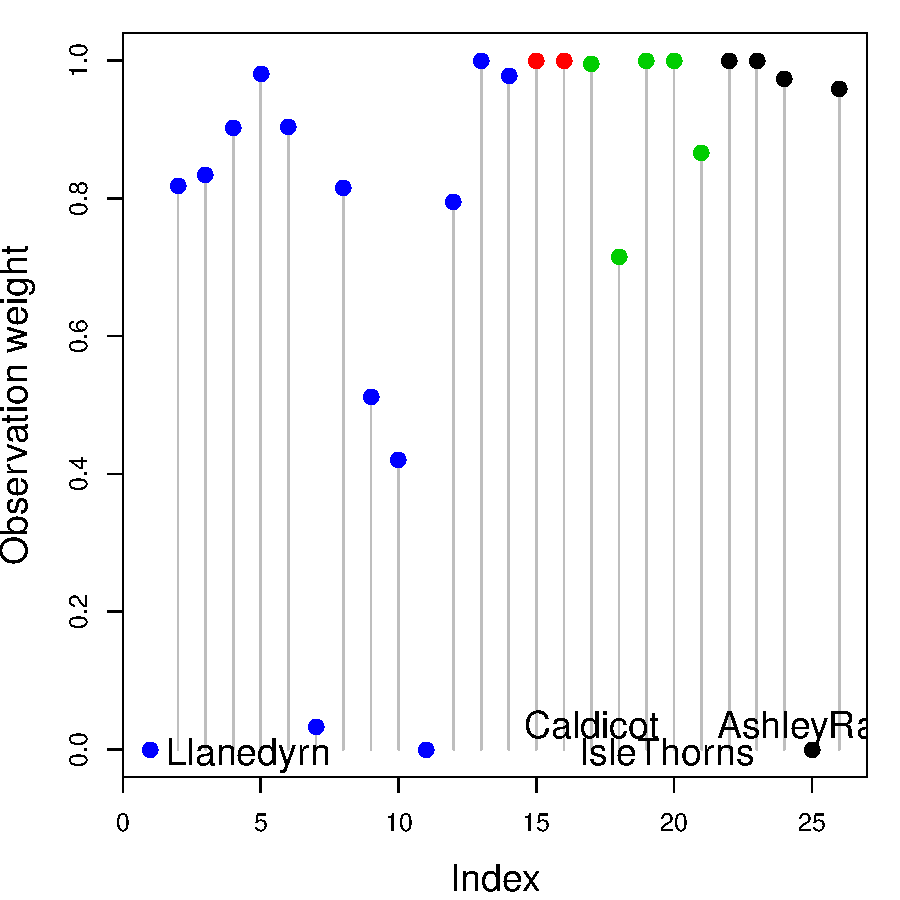
\includegraphics[width=1\linewidth,clip]{figures/pottery-weights}
   \end{minipage}%
  \hfill
  \begin{minipage}[c]{.5\textwidth}
   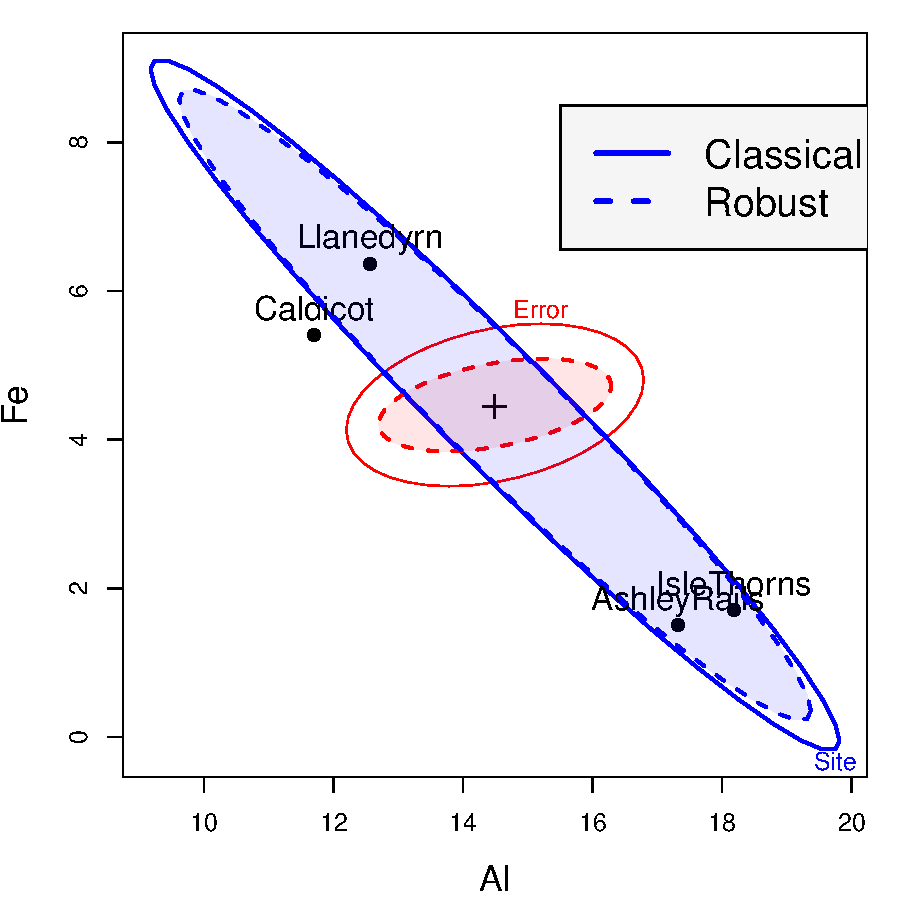
\includegraphics[width=1\linewidth,clip]{figures/pottery-robust}
  \end{minipage}

The $\mat{E}$ ellipse is considerably reduced, enhancing apparent significance 
\end{frame}
